% !TeX document-id = {759b9040-8a7f-4d09-8f16-a89e0a780c65}
%%% Magic comments for setting the correct parameters in compatible IDEs
% !TeX encoding = utf8
% !TeX program = pdflatex 
% !TeX spellcheck = en_US
% !BIB program = biber



\documentclass[notitlepage,english]{hgbreport}
%\usepackage{cmbright}
\usepackage{xfrac}
\usepackage{listings}
\usepackage[utf8]{inputenc}
\usepackage{cleveref}
\usepackage{wrapfig}
\usepackage{tcolorbox}

\usepackage{color, colortbl}
\definecolor{Gray}{gray}{0.925}
\renewcommand{\arraystretch}{1.15}


%acronyms
\newcommand{\Acronym}[1]{{#1}}
\newcommand{\LBP}{\Acronym{LBP}}
\newcommand{\SFM}{\Acronym{SFM}}


% names of things
\newcommand{\Python}{\textbf{Python}}
\newcommand{\JSON}{\textbf{JSON}}
\newcommand{\Numpy}{\textbf{NumPy}}
\newcommand{\Cupy}{\textbf{CuPy}}
\newcommand{\Pytorch}{\textbf{PyTorch}}
\newcommand{\OpenCV}{\textbf{OpenCV}}
\newcommand{\Github}{\textbf{GitHub}}
\newcommand{\ProjectUrl}{\url{www.github.com/giorgio-mariani/project1_IM_2018-2019}}
\newcommand{\ProjectDocUrl}{\url{\ProjectUrl/doc}}


%used boxes
\newenvironment{Note}
% env. opening
{
	\begin{tcolorbox}[title=Note:]
}
% env. closure
{ 
	\end{tcolorbox}
}

\newenvironment{FunctionBlock}
% env. opening
{	
	\begin{tcolorbox}[colback=green!5!white, colframe=green!60!black,title=Function:]
}
	% env. closure
{ 
	\end{tcolorbox}
}

\newenvironment{Important}
% env. opening
{
	\begin{tcolorbox}[colback=red!5!white, colframe=red!60!black,title=Important!]
	}
	% env. closure
	{ 
	\end{tcolorbox}
}


%--------------------
%-----
\DeclareMathAlphabet{\mathsfit}{T1}{\sfdefault}{\mddefault}{\sldefault}
\SetMathAlphabet{\mathsfit}{bold}{T1}{\sfdefault}{\bfdefault}{\sldefault}
\usepackage{bm}

%math notation
\renewcommand{\vec}[1]{\bm{\mathsfit{#1}}}
\newcommand{\mat}[1]{\bm{\mathsfit{#1}}}
\newcommand{\Transpose}[1]{#1^{\top}}
\newcommand{\Inverse}[1]{#1^{-1}}

\DeclareMathOperator*{\argmin}{argmin}
\DeclareMathOperator*{\argmax}{argmax}

\newcommand{\DataCostInit}{\mathop{\widetilde{E}_{data}}}
\newcommand{\DataCost}{\mathop{E_{data}}}
\newcommand{\ContinuityCost}{\mathop{E_{smooth}}}

\newcommand{\Vertices}{\mathcal{V}}
\newcommand{\Edges}{\mathcal{N}}
\newcommand{\Graph}{\mathcal{G}}

%---------------------------------------------
\lstdefinelanguage{JavaScript}{
	keywords={typeof, new, true, false, catch, function, return, null, catch, switch, var, if, in, while, do, else, case, break},
	keywordstyle=\color{blue}\bfseries,
	ndkeywords={class, export, boolean, throw, implements, import, this},
	ndkeywordstyle=\color{darkgray}\bfseries,
	identifierstyle=\color{black},
	sensitive=false,
	comment=[l]{//},
	morecomment=[s]{/*}{*/},
	commentstyle=\color{purple}\ttfamily,
	stringstyle=\color{violet}\ttfamily,
	morestring=[b]',
	morestring=[b]"
}

\lstset{
	language=JavaScript,
	extendedchars=true,
	basicstyle=\ttfamily,
	showstringspaces=false,
	showspaces=false,
	numbers=left,
	numberstyle=\footnotesize,
	numbersep=9pt,
	tabsize=2,
	breaklines=true,
	showtabs=false,
	captionpos=b
}
%-----------------------------------------------

\graphicspath{{images/}}  % where the images at?
\bibliography{references}  % requires file 'references.bib'

%%%----------------------------------------------------------
\author{Giorgio Mariani}										% your name
\title{IM490 Depth-Maps Recovery from an RGB-video\\	% the name of the course or project
				\textbf{Project 1 Report}}	% or "Project Report"
\date{\today}
%%%----------------------------------------------------------


%%%----------------------------------------------------------
\begin{document}
%%%----------------------------------------------------------

\maketitle

\begin{abstract}\noindent
	This report details the partial implementation of the depth-maps estimation procedure described by Zhang et al. in \cite{Zhang2009}, furthermore, an exhaustive explanation of said approach is given.
	More precisely, the addressed problem is the estimation of depth-maps from an RGB-video of a static scene. The original paper's main contribution is the expansion of a multi-view stereo approach with geometric coherence constraints, resulting in a method named \textit{Bundle Optimization}.  This addition allows the estimated depth-maps to be more stable when dealing with occlusion and disturbances in the source video.
	The implementation was mainly executed using the \Python{} programming language, expanded with vectorized computation libraries such as \Numpy{} and \OpenCV{}; for the latter the official python bindings were used.

%\bigskip
%\noindent
\end{abstract}


%%%----------------------------------------------------------
\tableofcontents
%%%----------------------------------------------------------




% TODO explain why OpenCV was chosen

%\subsection{Problems Encountered with OpenCV}


%%%----------------------------------------------------------

%%%----------------------------------------------------------
\chapter{Aims and Context}
%%%----------------------------------------------------------
\section{Introduction}\label{sec:introduction}
% describe problem
The aim of this project is the implementation of the article \textit{"Consistent Depth Maps Recovery from a Video Sequence"} \cite{Zhang2009}, by Zhang, Jia, Wong, and Bao and published in \textit{Transaction on Pattern Analysis and Machine Intelligence} (TPAMI).
%The article describes an algorithm which is able to generate a sequence of \emph{depth-maps} starting from an RGB-video.
The problem faced by Zhang et al. consists in estimating the {depth-maps}\footnote{A \emph{depth-map} is an image in which each pixel maintains depth information.} for all the frames contained in source RGB-video of a static scene.
More precisely, given an image sequence, the aim of the paper is to estimate a sequence of depth-maps having temporally consistent depth values.
This depth-maps can then be  used in several different of tasks; scene reconstruction and layer separation are two such examples. Having the depth values for all images in a video could also allow the usage of more sophisticated image processing techniques, an example could be the addition of virtual shadows in the source video.
\begin{figure}[!h]
	\centering
	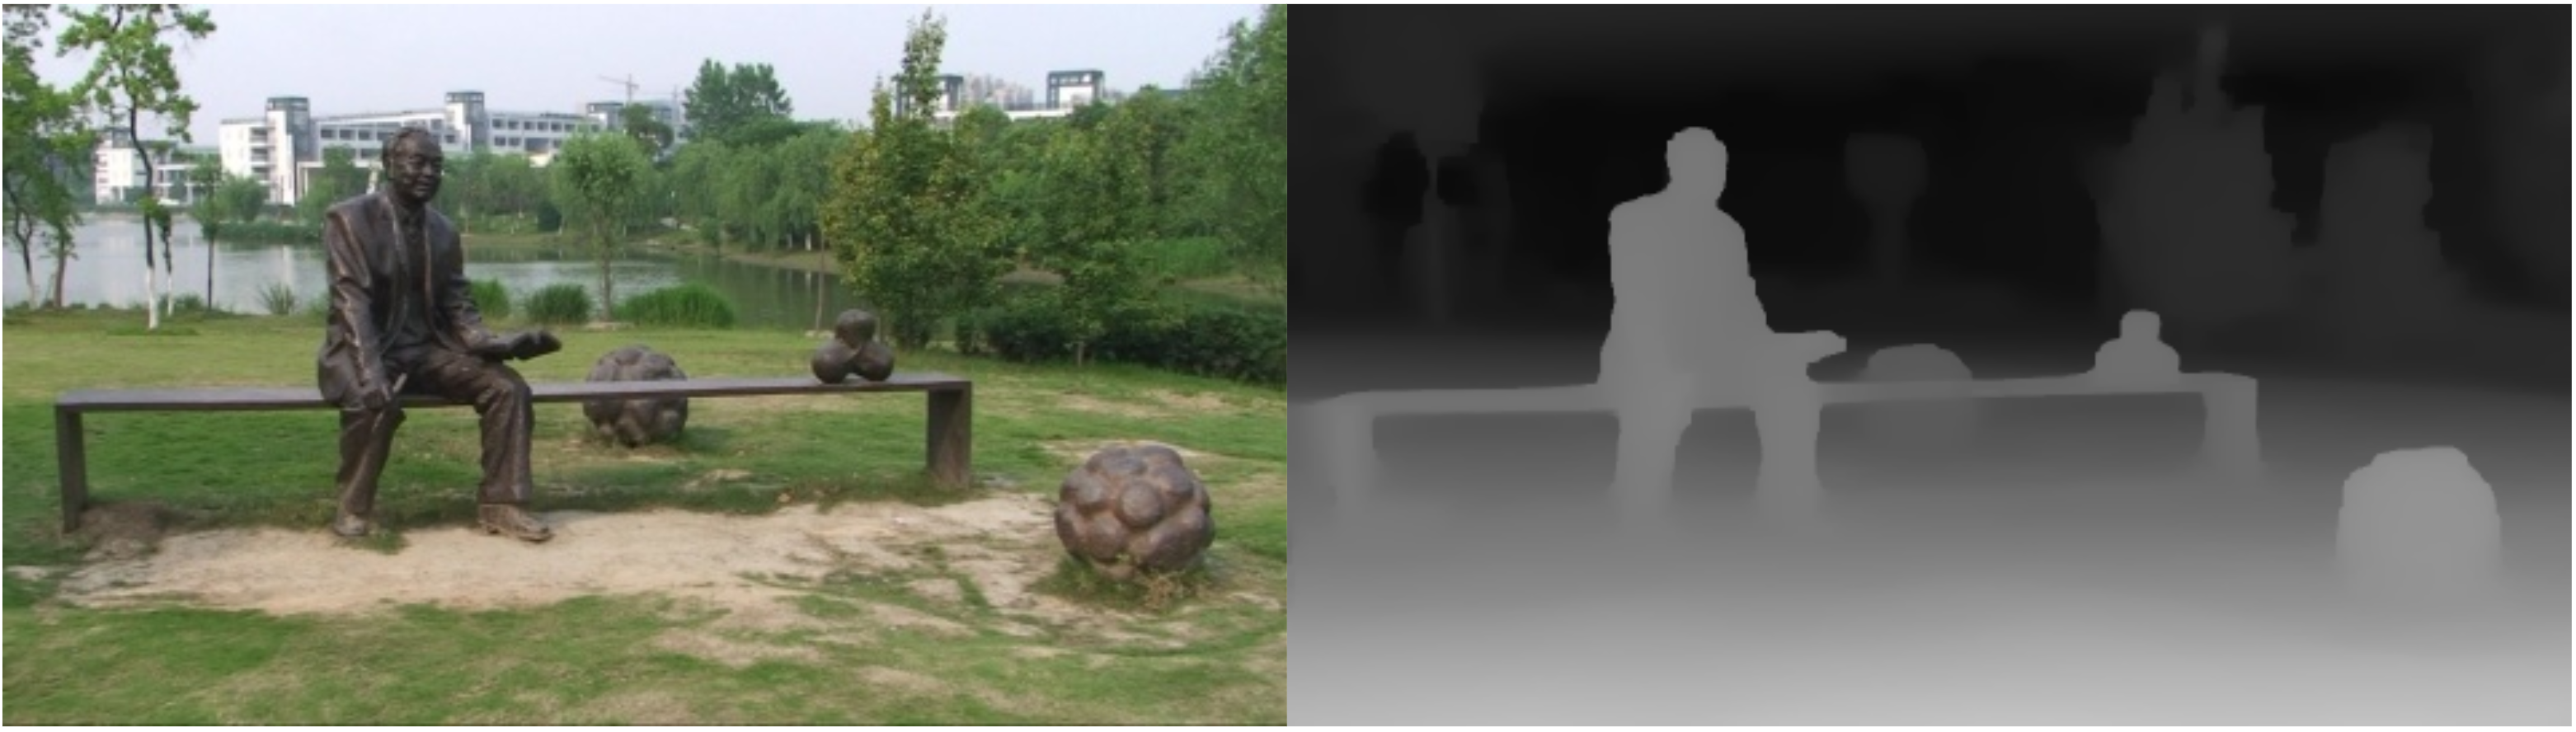
\includegraphics[width=.95\textwidth]{depthmap_example.png} %{CS0031}
	\caption{One of the estimated depth-maps  obtained using the approach described in \cite{Zhang2009} over a sequence of 200 images.}
\end{figure}
% TODO no explicit modeling of occlusion and noise
% TODO robust against noise
%One interesting feature of the approach in \cite{Zhang2009}
\begin{tcolorbox}[title=Note:]
While a free-of-charge implementation is available on the authors' website (\url{www.zjucvg.net}), they do not offer its source code; hence, the reasons behind this project are to offer an open-source implementation of said article, and to offer didactic improvement for the project's author.
This report's implementation can be found in the \Github{} repository
\ProjectUrl{}.
\end{tcolorbox}
%\footnote{See  Zhejiang University's {Computer Vision Group} website: \url{www.zjucvg.net}}

\section{Proposed Approach}
% overview of proposed solution
The approach proposed in the original article consists of four steps:
\begin{description}
\item\textbf{Camera Parameters Estimation.} During this phase, the camera parameters (\ie \emph{position}, \emph{rotation}, and \emph{intrinsic matrix}) are estimated using a \emph{Structure From Motion} (\SFM) algorithm. Unsurprisingly, the one used in the article is also related to a previous publication (see \cite{Zhang2007}) done by Zhang and Bao in collaboration with another research group. It is worth to note that \SFM{} algorithms can also produce as output a sparse cloud of 3D feature points (the ones used for the calibration). This is important since these points are also utilized during the depth-maps recovery. 
\begin{figure}[!h]
	\centering
	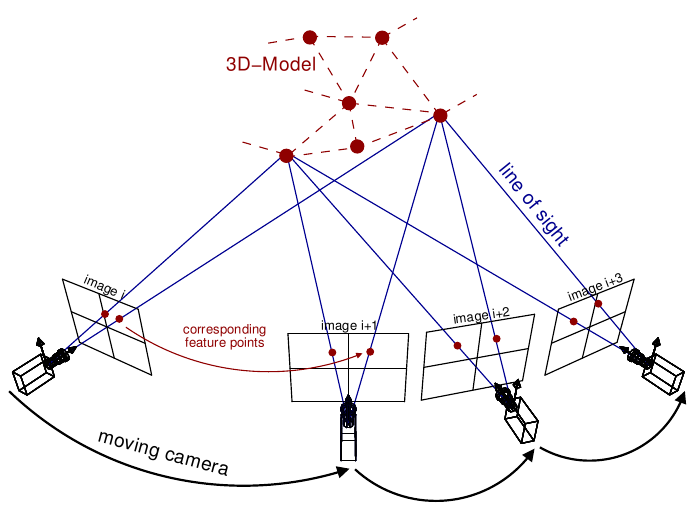
\includegraphics[width=.5\textwidth]{sfm.png} %{CS0031}
	\caption{SFM photo-grammetric approach; it tracks features points over different frames in order to infer the camera parameters. Source: \url{Theia-sfm.org}}
\end{figure}


\item\textbf{Disparity initialization.} 
For each frame in the video, a raw estimation of the corresponding depth-map is computed; this is achieved by minimizing an energy function whose parameters are the depth values to estimate.
These raw depth-maps are successively processed using a plane fitting algorithm: each image is divided into segments using \emph{mean-shift color segmentation} \cite{Comaniciu202}, these segments are then considered as a set of planes and fitted to the existing depth-maps raw values. The resulting images are the initialized depth-maps, ready to be used in the next step.

\item\textbf{Bundle Optimization.} The depth-maps obtained during the initialization process are then refined by applying geometric coherence constraints. This refinement process iteratively elaborates the given raw data by minimizing an energy function similar to the one used in the previous step, but enriched with geometric-consistency constraints.

\item\textbf{Space-Time Fusion.} This is the final step of the process, and it is used to polish the results obtained from the previous steps and removing eventual remaining noise.
The estimated depth-map values are used to define a loss function  that can subsequently be optimized through the use of iterative \emph{Conjugate Gradient Method}, an optimization technique able to find approximate solution to energy-minimization  problems.
The designed loss function takes into consideration: \emph{spatial continuity} between already computed depth-values, \emph{temporal coherence} of the estimated depth-maps, and consistency with the sparse points obtained by the \SFM{} algorithm used to compute the camera parameters.
\end{description}
 

%\section{Related Work}
%Since the proposed approach makes use of a variety of techniques, and it is relatively old (2009), the related work section is organized as follows:




%%%----------------------------------------------------------


\chapter{Complete Approach Description}

% in this section I will explain the implementation of each algorithm more in detail
 
 The goal of the system is to estimate a sequence of disparity-maps $\hat D = D_0, \dots, D_n$, using a sequence of images $\hat I = I_0, \dots, I_n$ and camera parameters.
 Specifically, for each image $I_t\in \hat I$ the camera's \emph{position}, \emph{rotation}, and \emph{intrinsic matrix} are assumed known, and are respectively noted as $\vec{T}_t$, $\mat{R}_t$, and $\mat K$ (note that the \emph{intrinsic matrix} does not depend on the frame).
 %TODO add explenation of estimation of camera parameters
 The estimated pixel $\vec x$'s disparity\footnote{The disparity of a certain pixel $\vec x$ correspond to the reciprocal of the pixel's depth ($\frac{1}{z_{\vec x}}$), however, the terms \emph{depth} and \emph{disparity} are sometimes used interchangeably.} at time $t$ is noted with $D_t(\vec x)$ (sometimes also referred to as $d_{\vec x}$ for shortness sake); the admissible disparity values used during the disparity-maps recovery are taken from the set $[d_{min}, d_{max}]$.
 
 %after its quantization into $m$ uniformly spaced values $d_{min}=d_0, \dots, d_{m-1} = d_{max}$. This disparity quantization is necessary in order to execute the algorithms utilized by the system. This is especially true for Belief Propagation, since it makes use of discrete labels instead of real values.

\section{Disparity Initialization}\label{sec:init_phase}
During the initialization phase, for each frame in the input video, an initial disparity-map is estimated; this estimation occurs within a two-step process: firstly, the depth-maps are initialized using a multi-view photo-consistency approach and \emph{Loopy Belief Propagation} (\LBP) \cite{Felzenszwalb2006}. Then, \emph{mean-shift segmentation}\cite{Comaniciu202} is employed over the sequence's images, dividing each picture into several segments similar in color. For each segment a "disparity plane" is thus fit to the image's disparity-map.

\subsection{Energy Minimization}
The initial disparity-maps estimation process works by minimizing the energy function
\begin{equation}
\label{eq:init_energy}
E_{init}(\hat D) = \sum_{t} \left(\DataCostInit(D_t) + \ContinuityCost(D_t)\right).
\end{equation}
The variable $t$ iterates over the video sequence frames, while the term $\DataCostInit(\cdot)$ indicates how much photo-consistent is the input depth-map $D_t$. Finally, $\ContinuityCost(\cdot)$ encodes how smooth\footnote{That is, how much difference there is between adjacent disparities.} the $D_t$ disparity-map is.\\

\begin{Important}
	The disparity values used during this estimation are quantized into $m$ uniformly spaced values $d_{min}=d_0, \dots, d_{m-1} = d_{max}$. This disparity quantization is necessary in order to execute the algorithms utilized by the system. This is especially true for Belief Propagation, since it makes use of discrete labels instead of real values.
\end{Important}

\paragraph{Energy Data Term.}
$\DataCostInit(\cdot)$ is defined in terms of \emph{disparity likelihood}, which in turn is defined as
$$L_{init}(\vec x, d) = \sum_{t'} p_c(\vec x,d,t,t').$$
This likelihood is used to the describe the photo-consistency of a certain disparity value $d$. Indeed, the function $p_c(\vec x,d,t,t')$ describes how much the pixel $\vec x$, using disparity $d$, is photo-consistent, which is expressed as
$$p_c(\vec x,d,t,t') = \frac{\sigma_c}{\sigma_c + \Vert I_t(\vec x) - I_{t'}(l_{t,t'}(\vec x,d))\rVert},$$
with $\sigma_c$ a constant value and $l_{t,t'}(\vec x,d)$ the projection of pixel $\vec x$ (taken from $I_t$) at time $t'$, using disparity $d$.
Finally, 
\begin{equation}\label{eq:init_energy_data}
\DataCostInit(D_t) = \sum_{\vec x} 1 -  u(\vec x) \cdot L_{init}(\vec x,D_t(\vec x)),
\end{equation}
with $u(\vec x)$ a normalization factor, such that the maximum value of the likelihood is 1; more precisely, it is true that $\max_{d} \{u(\vec x)\cdot L_{init}(\vec x, d)\} = 1$ (\ie the normalization is applied only with respect of the disparity value $d$ and not the pixel $\vec x$).

\paragraph{Energy Smoothness Term.}
The smoothness term $\ContinuityCost(D_t)$ is used to impose a smoother gradient during estimation.
This smoothness imposing strategy assigns an higher cost if two adjacent pixels have starkly different disparity-labels.
This label difference is measured using the function
$$\rho(d_{\vec x}, d_{\vec y}) = \min\{|d_{\vec x}-d_{\vec y}|, \eta\}.$$
The term $\eta$ is a real constant positive value, and it represents the upper limit of this smoothness imposing approach: after $\eta$ the distance between two labels does not matter during the energy minimization.

The value $\rho(\cdot)$ is then weighted using an adaptive smoothness weight $\lambda(\vec x, \vec y)$, which encodes changes of color between the adjacent pixels $\vec x$, $\vec y$: if $\vec x$ and $\vec y$ have strongly different colors in $I_t$ then the disparity smoothness requirement should be less strict, since they are less likely to be in a contiguous three-dimensional area. This is expressed as 
$$\lambda(\vec x,\vec y) = w_s\cdot \frac{u_\lambda(\vec x)}{|| I_t(\vec x) - I_t(\vec y)|| + \epsilon},$$
with $w_s$ a constant real positive value and $u_{\lambda}(\vec x)$ a normalization factor
$$
	u_{\lambda}(\vec x) = {|N(\vec x)|}\big/{\sum_{\vec y'\in N(\vec x)} \frac{1}{||I_t(\vec x) - I_t(\vec y')||+\epsilon}}.
$$
The smoothness term definition is then
\begin{equation}
	\ContinuityCost(D_t) = \sum_{\vec x} \sum_{\vec y\in N(\vec x)} \lambda(\vec x,\vec y)\cdot \rho(D_t(\vec x),D_t(\vec y)).
\end{equation}

%\paragraph{Minimization.}
%$E_{init}$ is then minimized using \LBP{}, process which requires a-priori the computation of an $h\times w\times m$ bi-dimensional table that stores the value
%$$1-u(\vec x)\cdot L_{init}(\vec x,d)$$ for each possible disparity-values $d$ and pixel $\vec x$. To see how this table is computed look at \cref{sec:init_phase_alg}.

\subsection{Disparity Planes Fitting}\label{sec:color_segmentation}
Using \emph{mean-shift segmentation}, it is possible to divide an image $I_t$ into different segments, which are then fitted to the initial estimation $D_t$:
\begin{enumerate}
\item First, the depth of the plane is selected by using the disparity that minimizes \cref{eq:init_energy}. The slope is assumed to be 0 during the fitting process.
\item Then, by using \emph{Levenberg-Marquardt algorithm}, the planes' slopes are estimated.
\end{enumerate}
These output planes represent the new refined depth-map, and are ready to be processed by the next phase of the algorithm.%(or used independently if precision is not that important)

\section{Bundle Optimization}\label{sec:bundle_phase}
\emph{Bundle optimization} is similar to the first step of the initialization phase, since it also makes use of consistency constraints and \LBP{} for disparity-maps polishing. However, the energy function to minimize is slightly different:
\begin{equation}
	E(\hat D) = \sum_{t} \left(\DataCost(D_t, \hat D) +
	\ContinuityCost(D_t)\right).
\end{equation}
The term $\ContinuityCost(\cdot)$ is the same as in \cref{eq:init_energy}, in contrast with $\DataCost(\cdot,\cdot)$, which substitutes $\DataCostInit(\cdot)$, and requires the sequence of initialized disparity-maps ($\hat D$). These  are then used to define geometry coherence constraints, which in turn will allow the estimation of more coherent and realistic disparity values.

The $\DataCost(\cdot, \cdot)$ terms is defined similarly to $\DataCostInit(\cdot)$, with only one major difference: the likelihood $L_{init}$ term is replaced by $L$, which is defined as
\begin{equation}\label{eq:bundle_energy_data}
L(\vec x, d) = \sum_{t'} p_c(\vec x,d,t,t')\cdot p_v(\vec x, d, D_{t'}),
\end{equation}
with $p_v$ the function used to encode geometric coherence:
\begin{equation} \label{eq:pv}
	p_v(\vec{x},d,D_{t^\prime}) = \exp \left(-\frac{\lVert \vec x - \mathop{l_{t',t}}(\vec x', D_{t'}(\vec x')) \rVert^2}{2\sigma^2_d}\right),
\end{equation}
with $\vec x'= l_{t,t'}(\vec x,d)$.
According to this definition, $p_v$ encodes the distance between the coordinates $\vec x$ and $l_{t',t}(\vec x', D_{t'}(\vec x'))$ using a gaussian distribution: the closer the two coordinates are, the higher $p_v$ is going to be; if they are the same, then it means that the depth values $d$ and $D_{t'}$ are geometrically coherent.



\section{Space-Time Fusion}\label{sec:spacetime_fusion}
While bundle optimization is able to improve the recovered disparity-maps obtained after disparity initialization, it is still not able to remove all the noise caused by the required disparity quantization and possible estimation errors; to solve this, a \emph{space-time fusion} algorithm is introduced in the recovery procedure. This further phase will polish the obtained results and provide smoother and real valued disparity-maps.
The space-time fusion will also exploit the sparse feature points generally obtained by \SFM{} algorithms in order to polish and enhance the disparity-maps.
This space-time fusion works by defining a number of constraints using the estimated disparity values $\{D_t\}_{t=0..n}$ in order to setup a linear system which is consequently solved using an iterative \emph{conjugate gradient solver}. The constraints used by the linear system can be divided into three categories:
\emph{spatial continuity}, \emph{temporal coherence}, and \emph{sparse feature correspondences}.
The solver resulting disparity-values are noted  as $\{D^*_t\}_{t=0..n}$.\\

\begin{Note}
In order to avoid severe memory consumption, space-time fusion is performed in batches of only 5-10 frames, instead of using the whole sequence.
\end{Note}


{
	%add newcommands
	\newcommand{\D}[1]{\mathop{D_{#1}}}
	\newcommand{\Dstar}[1]{\mathop{D^*_{#1}}}
	
	\subsection{Spatial Continuity}
	The depth structure of the recovered disparity-maps is generally correct, so it should be preserved in the fused disparity-maps. To do so, it is imposed that the difference between two neighboring pixels' disparities should mirror the one in the bundle disparity-maps.
	That is, for each frame $t$ and pixel $(x,y)$, the spatial constraints
	\begin{align*}
	\Dstar{t}(x+1,y) - \Dstar{t}(x,y)&=\D{t}(x+1,y) - \D{t}(x,y),\\
	\Dstar{t}(x, y+1) - \Dstar{t}(x,y)&=\D{t}(x,y+1) - \D{t}(x,y)
	\end{align*}
	are taken into consideration during the space-time fusion. 
	
	\subsection{Temporal Coherence}
	It is important for the estimated disparity-maps to be temporally coherent, that is, if a pixel $x$ has a certain disparity at frame $t$, then the same pixel projected at frame $t'$ (noted as $x'$) must have a coherent disparity values. This can be mathematically expressed, using epipolar geometry, through the formula
	\begin{equation}\label{eq:conj_pixel}
	\vec{x'} = 
	\Transpose{(x_{\vec x'} , y_{\vec x'} , z_{\vec x'} )} = 
	z_{\vec x} \Transpose{\mat R_{t'}} \mat R_{t} \mat K^{1}_{t'} \vec{x}^h + 
	\Transpose{\mat R_{t'}}(\vec T_t - \vec T_{t'}),
	\end{equation}
	where $\mat R$ is the rotation matrix, $\vec T$ the translation vector, and $\mat K$ is the intrinsic matrix.  It should also be noted, in order to avoid confusion, that $z_{\vec x}$ and $z_{\vec x'}$ are depth values, not disparities.

	It is then possible to simplify \cref{eq:conj_pixel} to 
	$z_{\vec x'} = \vec A\cdot z_{\vec x} + \vec B$,
	with $\vec A$ and $\vec B$ dependent on the pixel $\vec x$ and the camera parameters. This is useful, since it is able to give a direct correlation between the two depth values. 
	Indeed, if it is assumed that
	$$D^*_{t'}(\vec x') = \frac{1}{z_{\vec x'}}\text{ and }
	D^*_{t}(\vec x) = \frac{1}{z_{\vec x}},
	$$
	then it is possible to assert	
	\begin{equation*}
	\frac{1}{z_{\vec x'}} = \frac{1}{\vec A\cdot z_{\vec x} + \vec B} \iff
	D^*_{t'}(\vec x') = \frac{D^*_t(\vec x)}{\vec A + \vec B\cdot D^*_t(\vec x)},
	\end{equation*}
	which in turn can be used to define a temporal coherence constraint 
	over adjacent frames ($t$ and $t+1$), \ie
	\begin{equation}\label{eq:temp_constraint}
	\alpha \cdot \left( D^*_{t+1}(\vec x^{t\rightarrow t+1}) - \frac{D^*_t(\vec x)}{\vec A + \vec B\cdot D^*_t(\vec x)}\right) = 0.
	\end{equation}
	The vector  $\vec{x}^{t \leftarrow t+1}$ indicates the projection of pixel $x$ at time $t+1$ using disparity $D^*_{t}(\vec x)$, while the constant $\alpha$ is used to adjust the constraint's influence during estimation. In the experiments described in \cite{Zhang2009},  $	\alpha = 2$.\\

	\begin{Important}
		Since the used conjugate gradient solver requires linear constraints in order to work efficiently, \cref{eq:temp_constraint} is substituted by 
		\begin{equation*}
		\alpha \cdot\left( D^*_{t+1}(\vec x^{t\rightarrow t+1}) - \frac{D^*_t\left(\vec x\right)}{\vec A + \vec B\cdot \widetilde{D}^*_t(\vec x)}\right) = 0,
		\end{equation*}
		with $\widetilde{D}^*_t(\vec x)$ the value of ${D}^*_t(\vec x)$ in the previous iteration (or ${D}_t(\vec x)$ during the first iteration).
	\end{Important}
	%TODO include reliability of pixels
	
	{
	\newcommand{\ProjectedFeature}[2]{\vec{u}^{#1}_{\vec{#2}}}
	
	\subsection{Sparse Feature Correspondences}
 	During the camera parameters estimation (\SFM{} phase), it is possible to extract a set of sparse 3D feature points from the video. Hence, it is possible to exploit such feature points in order to guide the space-time fusion estimation process to more precise results. This is accomplished by projecting such points to a specific frame $t$ coordinate system, and  then imposing the feature point's depth to the corresponding pixel for frame $t$. 
 	
 	Having a 3D feature point $\vec X$ and a frame $t$, it is possible to compute its projection $\ProjectedFeature{t}{\vec X}$ using the equation
 	$$
 	\ProjectedFeature{t}{\vec X} = \mat{K}\Transpose{\mat{R}_t}\left(\vec X - \vec{T}_t\right),
 	$$
 	with $\mat{K}$, $\mat{R}_t$, and $\vec T_t$ the camera parameters.
 	The depth coordinate of $\ProjectedFeature{t}{\vec X}$ (noted as $d^{\vec X}_t$) is then used to add the constraint
 	\begin{equation}\label{eq:sparse_constraint}
 		\beta\cdot\left(D^*_t(\ProjectedFeature{t}{\vec X}) - d_t^{\vec X}\right) = 0.
 	\end{equation}
 	with $\beta=100$ used to adjust the constraint's influence during estimation. 
 	It is also important to note that constraints like \cref{eq:sparse_constraint} are used only for feature points $\vec X$ considered \emph{reliable}, that is, such that 
 	$\lVert D^*_t(\ProjectedFeature{t}{\vec X}) - d_t^{\vec X} \rVert < \kappa$, where $\kappa$ is a threshold.
 	}
}



%%%----------------------------------------------------------
\chapter{Project Details and Implementation}
%%%----------------------------------------------------------
\newcommand{\LongComment}[2]{\Comment{\parbox[t]{#1\linewidth}{#2}}}
%TODO say that broadcasting rules are used in algorithms
As already introduced, this project is a partial implementation of the article described in \cite{Zhang2009}. In this chapter it will be explained more in detail \emph{what} and \emph{how} was everything implemented.
%, starting from the architecture used by the system, to the pseudo-code of the implemented algorithms.
The decision to not do a complete implementation of the system was adopted due to the following reasons:
\begin{itemize}
\item Reduced time on the author's part, which rendered the completion of some section of the paper not plausible. 
\item Inexperience in some field of study necessary to the implementation of some part of the system, namely \emph{Conjugate Gradient Method} in the space-time fusion phase  (\cref{sec:spacetime_fusion}).
\item Difficult compatibility of used technology for some of the faced problems, \ie{} mean shift segmentation (\cref{sec:color_segmentation}) using the python's \OpenCV{} binding was more  burdensome to implement than expected.
\end{itemize}


\section{The Architecture}
The systems is written using the \emph{Python Programming Language}; the reason behind this decision is the relative good performance that vectorized computation libraries can achieve on python, the flexibility and simplicity of the language, and the author's past experience with python libraries such as \textbf{NumPy} and \textbf{TensorFlow}, which makes the development less laborious.
%TODO say python version

\subsection{Dependencies and Third Party Libraries}
\paragraph{NumPy:} The main library used for computations in the project is the \textbf{NumPy} module: it is a set of function designed for intensive computing in vectorized fashion, similarly to the \textbf{MATLAB} programming language.

\paragraph{OpenCV:}
The \textbf{OpenCV} library (version 4.0.0) is also utilized in the project, using the official python bindings.
\textbf{OpenCV} offers real-time computer vision by exploiting (whenever possible) accelerated hardware, such as GPUs.
Unfortunately, the official bindings are available only for python 2.7.\textit{x} interpreters, forcing the author to use a compatible interpreter.


\section{Implementation}
In this section the various algorithms employed by the system and  implemented for the project are explained through the use of pseudo-code. To get a more in-depth look at how the system works, the reader should refer to the project's \Github{} repository at \ProjectUrl.

\subsection{Implemented Components}\label{sec:implemented components}
The parts of the system described in \cite{Zhang2009} that were de-facto implemented are the following:
\begin{itemize}
	\item Disparity Initialization (\cref{sec:init_phase}) without the color segmentation/disparity plane fitting component, \ie{} only the \LBP{} optimization part is used for initializing the disparity-maps.
	\item Bundle Optimization (\cref{sec:bundle_phase}), which was entirely implemented.
\end{itemize}
In other words, the omitted parts are both the second step of the initialization phase and the space-time fusion of the bundle results.

Furthermore, the camera parameters are assumed known; this should not be a restricting assumption since there is rich literature in terms of camera calibration and parameters estimation, and a variety of algorithms, such as the one described in \cite{Zhang2007}, can be employed in order to solve this known problem.

\subsection{Notation}
In this section, some guidelines on how to read the pseudo-code are defined:
%For example, different fonts are used depending on the nature of the represented variable.
\begin{itemize}
	\item Matrices and vectors are noted using bold serif font: $\mat M$,  $\vec x$, e.t.c.
	\item Sequences of objects are noted using calligraphic font:  $\mathcal{I}$, $\mathcal{D}$, e.t.c.
	\item The notation $3\times 4 \times 5$ indicates the shape of array with three elements in the first dimension, four in the second one, and five in the last one.
	\item Functions of type \texttt{reduce\_\textit{func}(\textit{array},\textit{axis})} apply the reduce function \texttt{\textit{func}} ($\min$ for example) over the dimension at position \texttt{\textit{axis}}.
	\item Functions of type \texttt{elementwise\_\textit{func}(\texttt{\textit{array}})} apply the function \texttt{\textit{func}} to each element in \texttt{\textit{array}}.
	\item The function \texttt{reshape(\textit{array}, \textit{shape})} reshapes \texttt{\textit{array}} to the shape \texttt{\textit{shape}}.
\end{itemize}


\subsection{Loopy Belief Propagation}
As already mentioned, \LBP{} is an optimization technique that can be used in order to approximate minimal graph labelings. For a more in-depth description of the algorithm see \cref{app:LBP}. In this section, the pseudo-code of the implementation used in this project is shown. It should be mentioned that the given code (for simplicity sake) does only partially  reflect the actual implementation, since some optimizations and complications (like the smoothness factor $\lambda(\cdot,\cdot)$ and the Multiscale variant of \LBP{}) are not present.\\
\begin{Note}
	In order to understand this section, the reader is strongly suggested to  first read \cref{app:LBP}.
\end{Note}

\begin{algorithm}[H]
\caption{Loopy Belief Propagation}\label{alg:lbp}
\begin{algorithmic}[1]
\Require{$\mat D$ has shape $h\times w \times k$.}\Comment{Data Cost}
\Require{$s>0$ and $\eta\ge0$.}
\Statex
\Procedure{LBP}{$\mat D$, $s$, $\eta$}
\State Create $\mat{m_\mathit{x}}$ with shape $h\times w\times k$ (init. to zero). \Comment{$\forall \mat{\mathit x}\in\{\mat{up},\mat{down}, \mat{left}, \mat{right}\}$}
\Statex
\For{${t}\leftarrow 0,\dots, T$}
	\State $\mat{h_{tot}} \leftarrow \mat D + \mat{m_{up}} +\mat{m_{down}} + \mat{m_{left}} + \mat{m_{right}}$
	\State $\mat{h_{up}} \leftarrow \texttt{moveDown}(\mat{h_{tot}}-\mat {m_{down}})$\label{ist:h_start}\Comment{Start computing $h(f)$}
	\State $\mat{h_{down}} \leftarrow \texttt{moveUp}(\mat{h_{tot}}-\mat {m_{up}})$
	\State $\mat{h_{left}} \leftarrow \texttt{moveRight}(\mat{h_{tot}}-\mat {m_{right}})$
	\State $\mat{h_{right}} \leftarrow \texttt{moveLeft}(\mat{h_{tot}}-\mat {m_{left}})$\label{ist:h_end}\Comment{Finish computing $h(f)$}
	\Statex
	\For { $\mat x \in \{\mat{up}, \mat{down}, \mat{left}, \mat{right}\}$}		\label{ist:start_thing}\Comment{Start computing $m(f)$}
		\State $\mat {m_x} \leftarrow \mat{h_x}$
		\For{ $i=0,\dots,k$}
		\State $\mat{m_x} \leftarrow \min\left( \mat{m_x}[:, :, i], \mat{m_x}[:, :, i-1] + s\right)$
		\EndFor
		\For{ $i=k,\dots,0$}
				\State $\mat{m_x} \leftarrow \min\left( \mat{m_x}[:, :, i], \mat{m_x}[:, :, i+1] +  s\right)$\Comment{Finish computing $m(f)$}
		\EndFor 
	\EndFor
	\Statex
	\For { $\mat x \in \{\mat{up}, \mat{down}, \mat{left}, \mat{right}\}$}
		\State $\mat{tmp}\leftarrow$\texttt{reduce\_min}($\mat{h_x}$, \textit{last-axis})$+\eta$ \Comment{$\mat{tmp}$ has shape $h\times w$}
		\State $\mat{m_x} \leftarrow \texttt{elmentwise\_min}\left(\mat{m_x}, \mat{tmp}\right)$
		\label{ist:end_thing}
		\LongComment{.32}{$\mat{tmp}$ is broadcast to shape $h\times w \times k$}
	\EndFor
\EndFor
\Statex
\State $\mat B \leftarrow$ Copy of $\mat D$ 
\For {$\mat x \in \{\mat{up}, \mat{down}, \mat{left}, \mat{right}\}$} \Comment{Compute belief vector}\label{istr:belief_comp1}
	\State $\mat B \leftarrow \mat B+\mat{m_x}$\label{istr:belief_comp2}
\EndFor
\State \Return \texttt{reduce\_argmin}($\mat B$, \textit{last-axis})\Comment{output labels, shape: $h\times w$}
\EndProcedure
\end{algorithmic}
\end{algorithm}

The \LBP's pseudo-code can be observed in \cref{alg:lbp}. 
The input parameter $\mat D$ represents the \emph{data cost} term in \cref{eq:lbp:energy}, while the values $s$, $\eta$ represent the homonymous constants in \cref{eq:lbp:discontinuity}. $\mat D$ is a multi-dimensional array having shape $h\times w \times k$, with  $k$ the number of utilized labels. The value $v$ at position $\mat D[x,y,f]$ indicates the data cost for label $f$ at pixel $(x,y)$.\\

\begin{FunctionBlock}
	The class of functions \texttt{move\textit{Direction}($\mat M$)} move (by one position) all elements in the input matrix with respect to the direction expressed by \texttt{\textit{Direction}}. In practical terms, an affine transformation is applied over $\mat M$.
\end{FunctionBlock}

The sent messages $m^t_{(\vec p,\vec q)}$ are implemented through the matrices $\mat{m_{up}}$,  $\mat{m_{down}}$, $\mat {m_{left}}$, and $\mat{m_{right}}$. Each of these has shape $h\times w \times k$ and represents $m^t_{(\vec p,\vec q)}$ with respect to edges in one of the possible four directions. For example,
$$\mat{m_{up}}[y,x] = m^t_{\left((x,y+1), (x,y)\right)}.$$

%The computation of $h(f)$ is performed in l
The code between \cref{ist:start_thing} and \cref{ist:end_thing} implements the \cref{eq:lbp:update2}, while computation of the \emph{belief vectors} is done at lines \ref{istr:belief_comp1} and \ref{istr:belief_comp2} by summing $\mat{m_{up}}$,  $\mat{m_{down}}$, $\mat {m_{left}}$, and $\mat{m_{right}}$ to $\mat D$.
 Finally, the output disparity-labels are calculated in the last line of the procedure by extracting from $\mat B$'s last dimension (which contains label indeces) the labels having minimal weights.

\subsection{Disparity Initialization}\label{sec:init_phase_alg}
In order to minimize the energy function described in \cref{eq:init_energy}, the \LBP{} algorithm (see above) is used.
For the disparity-map recovery problem, the disparity-map is expressed as a grid graph (with each node representing a pixel and having at most four adjacent nodes), and the possible labels are the disparity values $d_0,\dots,d_{m-1}$. Therefore, an assignment of these labels over the graph's nodes is a possible disparity-map.

In order to work, the \LBP{} algorithm requires as input the \emph{data cost}, \ie{} the cost of assigning a disparity value to a pixel $\vec x =(x,y)$, for all pixels.
This cost is  specified by \cref{eq:init_energy_data}, particularly for every pixel $\vec x$ and disparity label $d$, the value 
$$1 - u(\vec x)\cdot L_{init}(\vec x, d)$$ should be computed. The value $u(\vec x)\cdot L_{init}$ is essentially the likeliness (normalized through $u(\vec x)$) of a pixel to have disparity $d$. 

Computation of the disparity data cost is done through \cref{alg:energy_data_init}.
The algorithm takes as input a frame $t$, the camera parameters (denoted by $\mat K$, $\mathcal R$, and $\mathcal T$), and the image sequence $\mathcal{I}$ and outputs a multi-dimensional array with shape $h\times w \times m$ representing the data cost for the disparity-map estimation problem.

Procedure \texttt{conjugate\_coor}, described in \cref{alg:conjugate_coor}, computes for each homogeneous coordinate in the array $\mat x^h$, the respective conjugate point w.r.t. the given camera parameters and depth values. This procedure is a vectorized implementation of the formula in \cref{app:conjugate_pixel}.

\begin{algorithm}
	\caption{\texttt{compute\_energy\_data\_init}}
	\label{alg:energy_data_init}
               
	\begin{algorithmic}[1]
		\Require $\mat K$ to be the camera intrinsic matrix
		\Require $\mathcal{R}$ to be a sequence of camera rotation matrices
		\Require $\mathcal{T}$ to be a sequence of camera translation vectors
		\Require $\mathcal{I}$ to be a sequence of images
		\Statex
		\Procedure{compute\_energy\_data\_init}{$t$, $\mat K$, $\mathcal{R}$, $\mathcal{T}$, $\mathcal{I}$}		

		\State $\mat {I_t}$, $\mat {R_t}$, $\mat {T_t} \leftarrow \mathcal{I}[ t ]$, $\mathcal{R}[t]$, $\mathcal{T}[t]$\Comment{get image and camera param. for frame $t$}
		\State $\vec x^h \leftarrow$ \texttt{homogeneous\_coor\_grid}($h$,$w$)\Comment{create a grid of hom. indices}
		\State Create table $\mat L$ with $h \times w\times m$ elements (init. to zero).
		%\State L $\leftarrow$ $m\times h \times w$ table, initialized with zero
		\Statex
		\For {$t'\leftarrow 0\dots n$}
		\State $\mat{I_{t'}}$, $\mat {R_{t'}}$, $\mat {T_{t'}} \leftarrow \mathcal{I}[ t' ]$,  $\mathcal{R}[t']$, $\mathcal{T}[t']$\Comment{get image and camera param. for frame $t'$}
		\Statex
		\For {${label} \leftarrow 0\dots m$}
		\State Create matrix $\mat D$ with $h \times w$ elements, initialized with value $d_{label}$
		%\State $\mathrm{d}[i,j] \leftarrow \mathrm{depth\_values}[level]$, $\forall i,\forall j$
		\State $\vec{x'}^h\leftarrow$ \texttt{conjugate\_coor}($\vec x^h$, $\mat K$, $\mat{R_{t}}$, $\mat{R_{t'}}$,  $\mat{ T_{t}}$, $\mat{ T_{t'}}$, $\mat D$)
		\State $\mat{I^r_{t'}} \leftarrow$ \texttt{remap}($\mat{I_{t'}}$, $\vec{x'}^h$)
		\State $p_c \leftarrow$  $\sigma_c$ / $(\sigma_c +$ \texttt{reduce\_norm($\mat{I_t} - \mat{I^r_{t'}}$)})
		\State $\mat L[:,:,label] \leftarrow \mat L[:,:label] + p_c$\Comment{likeliness for label $label$}
		\EndFor
		\EndFor
		\Statex
		\State $\mat u \leftarrow$ $1$/ \texttt{reduce\_max}($\mat L$, \textit{last-axis})\Comment{normalization factor w.r.t. to label axis}
		\State \Return $1 - \mat u\cdot \mat L$
		\EndProcedure
	\end{algorithmic}
\end{algorithm}
%\begin{figure}[!h]
%	\centering
%	\begin{tabular}{|l  l|}\hline\hline
%		\textbf{variable}&\textbf{shape}\\
%		$x^h$, $x'^h$&  $3\times h\times w$\\
%		$D$ & $h\times w$\\
%		$I_t$, $I_{t'}$, $I^p_{t'}$&$h\times w$\\
%		$L$&$m\times h \times w$\\
%		$p_c$, $u$&$h\times w$\\\hline\hline
%	\end{tabular}
%	\caption{Shapes of the variables in \cref{alg:energy_data_init} }
%\end{figure}
\begin{algorithm}
	\caption{\texttt{conjugate\_coor}}
	\label{alg:conjugate_coor}
	
	\begin{algorithmic}[1]
		\Procedure{conjugate\_coor}{$\vec x^h$, $\mat K$, $\mat{R_{1}}$, $\mat{R_{2}}$,  $\mat{ T_{1}}$, $\mat{ T_{2}}$, $\mat D$}	
		\State \texttt{reshape}($\mat{x}^h$, $3\times (h\cdot w)$) \Comment{reshape for matrix mul.}
		\State \texttt{reshape}($\mat{D}$, $1\times(h\cdot w)$)\Comment{reshape for matrix mul.}
		\State $\mat {x'}^h \leftarrow \mat K\Transpose{\mat{R_2}}\cdot\left(
			\mat{R_1}\Inverse{\mat K}\vec x^h + 
			\Transpose{(\mat{T_1}-\mat{T_2})} \cdot \mat D
		\right)$
		\State \texttt{reshape}($\mat{x'}^h$, $3\times h\times w$) \Comment{go back to normal shape}
		\EndProcedure
	\end{algorithmic}
\end{algorithm}

\begin{FunctionBlock}
The procedure \texttt{homogeneous\_coordinate\_grid($h$, $w$)} produces a multi-dimensional array $\vec x^h$ filled with a grid of homogeneous coordinates, such that the first axis represent the coordinate itself, \ie
\begin{align*}
\vec x^h[0,i,j] &= i\\
\vec x^h[1,i,j] &= j\\
\vec x^h[2,i,j] &= 1
\end{align*}
The coordinates assume integer values between $0$ to $h$ (excluded) for the second axis (that is, value $i$ in above equation) and between $0$ and $w$ (excluded) for the third axis (value $j$). Consequently, $\vec x^h$'s shape is $3\times h \times w$.
\end{FunctionBlock}

\begin{FunctionBlock}
The procedure \texttt{remap($\vec I$, $\mat{map}$)} is used to transform the input image $\vec I$ using a certain mapping $\mat{map}$ such that the output image $\vec{I'}$ is defined as  
$$\vec{I'}[\vec x] = \vec I[\mat{map}[\vec x]].$$
%The reader should note that in \cref{alg:energy_data_init} there is an abuse of notation, since the variable $\vec{x'}^h$ (which assumes role of the argument $\mat{map}$ in the function call) has shape $3\times h \times w$ instead of the required $h\times w \times 2$; however, this can be easily solved by transforming $x'^h$ to the non-homogeneous coordinates $x'$ and then transposing it. 
\end{FunctionBlock}

\subsection{Bundle Optimization}
As with Disparity Initialization, Bundle Optimization makes also use of \LBP{} in order to estimate the disparity-maps. 
As a result, the algorithm used for Bundle Optimization is similar to the one used to compute the data cost during the disparity initialization (see \cref{alg:energy_data_init}), the only major difference is the requirement to compute the term $p_v$, found in \cref{eq:pv}. This term is indeed used in order to define the Bundle Optimization likelihood (function $L$ in \cref{eq:bundle_energy_data})
%for the first step of the initialization phase (\cref{sec:init_phase}), the only major difference is in the computation of the term $p_v$, which is multiplied to $p_c$ before updating the likelihood $L$. 
By adding the pseudo-code at \cref{alg:compute_pv} in the inner for loop and by changing how the array $\mat L$ is updated, it is possible to expand \cref{alg:energy_data_init} with Bundle Optimization.
The use of such component is managed by the boolean variable $use\_bundle$.
Thus, the final algorithm, able to exploit the term geometric coherence constraint $p_v$, is described in \cref{alg:energy_data}. 
%Note that the functions \texttt{homogeneous\_coordinate\_grid}, \texttt{conjugate\_coor}, \texttt{remap},  \texttt{norm}, and  \texttt{reduce\_max} work as described in \cref{sec:init_phase_alg}.
\begin{algorithm}[H]
	\caption{\texttt{compute\_pv}}
	\label{alg:compute_pv}
	\begin{algorithmic}[1]
		\Procedure{conjugate\_coor}{$\vec {x'}^h$, $\mat K$, $\mat{R_{1}}$, $\mat{R_{2}}$,  $\mat{ T_{1}}$, $\mat{ T_{2}}$, $\mat D$}	
		\State $\mat{D^r} \leftarrow$ \texttt{remap}($\mat{D}$, $\vec{x'}^h$)
		\State $\vec{l_{t',t}}\leftarrow$ \texttt{conjugate\_coordinates}($\vec {x'}^h$, $\mat K$, $\mat{R_{2}}$, $\mat{R_{1}}$,  $\mat{ T_{2}}$, $\mat{ T_{1}}$, $\mat D^r$)
		\State \Return $\exp\left(-{\lVert \vec x - \vec{l_{t',t}}\rVert^2}\cdot\frac{1}{2\sigma_d^2}\right)$
		\EndProcedure
	\end{algorithmic}
\end{algorithm}
\begin{algorithm}
	\caption{\texttt{compute\_energy\_data}}
	\label{alg:energy_data}	
	\begin{algorithmic}[1]
		\Require $\mat K$ to be the camera intrinsic matrix
		\Require $\mathcal{R}$ to be a sequence of camera rotation matrices
		\Require $\mathcal{T}$ to be a sequence of camera translation vectors
		\Require $\mathcal{I}$ to be a sequence of images
		\Require $\mathcal{D}$ to be a sequence of disparity-maps
		\Statex
		\Procedure{compute\_energy\_data\_init}{$t$, $\mat K$, $\mathcal{R}$, $\mathcal{T}$, $\mathcal{I}$, $\mathcal{D}$}		

		\State $\mat {I_t}$, $\mat {R_t}$, $\mat {T_t} \leftarrow \mathcal{I}[ t ]$, $\mathcal{R}[t]$, $\mathcal{T}[t]$\Comment{get image and camera param. for frame $t$}
		\State $\vec x^h \leftarrow$ \texttt{homogeneous\_coor\_grid}($h$,$w$)
		\State Create table $\mat L$ with $h \times w\times m$ elements, initialized with zero
		%\State L $\leftarrow$ $m\times h \times w$ table, initialized with zero
		\Statex
		\For {$t'\leftarrow 0\dots n$}
		\State $\mat{I_{t'}}$, $\mat {R_{t'}}$, $\mat {T_{t'}} \leftarrow \mathcal{I}[ t' ]$,  $\mathcal{R}[t']$, $\mathcal{T}[t']$\Comment{get image and camera param. for frame $t'$}
		\Statex
		\For {${label} \leftarrow 0\dots m$}
		\State Create matrix $\mat D$ with $h \times w$ elements, initialized with value $d_{label}$
		%\State $\mathrm{d}[i,j] \leftarrow \mathrm{depth\_values}[level]$, $\forall i,\forall j$
		\State $\vec{x'}^h\leftarrow$ \texttt{conjugate\_coor}($\vec x^h$, $\mat K$, $\mat{R_{t}}$, $\mat{R_{t'}}$,  $\mat{ T_{t}}$, $\mat{ T_{t'}}$, $\mat D$)
		\State $\mat{I^r_{t'}} \leftarrow$ \texttt{remap}($\mat{I_{t'}}$, $\vec{x'}^h$)
		\State $p_c \leftarrow$  $\sigma_c$ / $(\sigma_c +$ \texttt{reduce\_norm($\mat{I_t} - \mat{I^r_{t'}}$)})
		\If {use\_bundle}\Comment{Check if Bundle Optimization}
		\State $p_v \leftarrow $\texttt{compute\_pv}($\vec x^h$, $\mat K$, $\mat{R_{t}}$, $\mat{R_{t'}}$,  $\mat{ T_{t}}$, $\mat{ T_{t'}}$, $\mathcal D[t']$)
		\State $\mat L[:,:,label] \leftarrow \mat L[:,:label] + p_c\cdot p_v$\Comment{likeliness for label $label$}
		\Else
		\State $\mat L[:,:,label] \leftarrow \mat L[:,:label] + p_c$\Comment{likeliness for label $label$}
		\EndIf
		\EndFor
		\EndFor
		\Statex
		\State $\mat u \leftarrow$ $1$/ \texttt{reduce\_max}($\mat L$, \textit{last-axis})\Comment{normalization factor w.r.t. to label axis}
		\State \Return $1 - \mat u\cdot \mat L$
		\EndProcedure
	\end{algorithmic}
\end{algorithm}



%%%----------------------------------------------------------     
\chapter{System Documentation}
%%%----------------------------------------------------------
%Give a well-structured description of the architecture and the technical design of your implementation, with sufficient granularity to enable an external person to continue working on the project.
\newcommand{\ComputeEnergy}{\texttt{compute\_energy}}
\newcommand{\Estimate}{\texttt{estimate}}
\newcommand{\Lbp}{\texttt{lbp}}
\newcommand{\Utils}{\texttt{utils}}
\newcommand{\Params}{\texttt{params}}

\section{Dependencies Installation}
%show how to install opencv and various requirements
The system makes use of several external libraries, which can be easily installed using \texttt{pip} and the \texttt{requirements.txt} file:
\begin{lstlisting}[stepnumber=0]
pip install -r requirements.txt
\end{lstlisting}
\begin{tcolorbox}[title=Note:]
\textbf{Python 2.7} is required in order to run the system, consequently, the appropriate version of \textbf{pip} should be used. 
\end{tcolorbox}

\section{Running the System}
%In order to estimate the depth-map of a 
The system can be executed by invoking the following instruction from the operating system's command line terminal:
\begin{lstlisting}[stepnumber=0]
	python estimate.py [-i][-b] <config.txt>
\end{lstlisting}
The argument \texttt{<config.txt>} is a configuration file containing parameter values and paths to the folder storing all data necessary for the disparity-maps recovering process (this data is generally either pictures or other disparity-maps).
The options \texttt{-i} and \texttt{-b} are used to communicate the system which  of the available phase should be executed:
\begin{description}
	\item[\texttt{-i}] it executes only Disparity Initialization; the resulting disparity-maps are then stored in an output folder.
	\item[\texttt{-b}] it executes only Bundle Optimization. Note that ,because of how bundle optimization works, it also requires as input  the previously estimated depth-maps. As before, the resulting disparity-maps are then stored in an output folder.
	\item[\texttt{-ib}] it executes both Disparity Initialization and Bundle Optimization.
\end{description}

\section{System's Input}
\newcommand{\ConfigParam}[1]{\texttt{"#1"}}

\subsection{Camera File}
This file contains information about the camera parameters; in particular, it stores information 
about intrinsic matrix, rotations, and translation of the camera for each picture in the sequence.
The camera file itself is quite simple; for each image the intrinsic matrix, 
rotation matrix, and position must be included in plain text, one after the other, without interleaving blank lines.

The code below shows an example of such format: the first three rows are the \emph{intrinsic matrix},
the second three rows are the \emph{rotation matrix}, and the final row is the \emph{position vector}.
\begin{lstlisting}[language=C]
1139.7929     0.0000000     479.50000
0.0000000     1139.7929     269.50000
0.0000000     0.0000000     1.0000000
1.0000000     0.0000000     0.0000000
0.0000000     1.0000000     0.0000000
0.0000000     0.0000000     1.0000000
0.0000000     0.0000000     0.0000000
\end{lstlisting}
\dotfill

This pattern must be repeated for each image in the target sequence, and two blank lines must be used between data of different images.
Also, the first line of the camera file must be a number, indicating the number of camera frames in the file itself. A blank line must follow. A complete example of a camera file which makes use of a sequence with three frames is the following:
\begin{lstlisting}[language=C]
3

1139.7929     0.0000000     479.50000
0.0000000     1139.7929     269.50000
0.0000000     0.0000000     1.0000000
1.0000000     0.0000000     0.0000000
0.0000000     1.0000000     0.0000000
0.0000000     0.0000000     1.0000000
0.0000000     0.0000000     0.0000000


1139.7929     0.0000000     479.50000
0.0000000     1139.7929     269.50000
0.0000000     0.0000000     1.0000000
0.9999972     -0.001567     0.0017456
0.0015681     0.9999985     -0.000634
-0.001744     0.0006373     0.9999982
-0.320146     0.0141622     -0.049300


1139.7929     0.0000000     479.50000
0.0000000     1139.7929     269.50000
0.0000000     0.0000000     1.0000000
0.9999884     -0.002738     0.0039581
0.0027459     0.9999945     -0.001806
-0.003953     0.0018177     0.9999905
-0.720470     -0.028543     -0.089562
\end{lstlisting}
\dotfill
\begin{Note}
The location of the camera file is defined by the configuration parameter 
\ConfigParam{camera\_file}.
\end{Note}


\subsection{Pictures Directory}
Directory which contains the picture sequence to be used during the estimation process.
The images must be named using the syntax \texttt{img\_<num>}, with \texttt{<num>} numeric string with value in the range between \texttt{0000} ang \texttt{9999}. The images filenames must be organized in a 
contiguous fashion: no gaps should be present between the smallest and largest filename numbers.
All such image files should have same format and resolution.\\
\begin{Note}
The image format, as well as the location of the directory are indicated by the configuration parameters
\ConfigParam{pictures\_file\_extension} and\ConfigParam{pictures\_directory} respectively. 
\end{Note}

\subsection{Depth-maps Directory}\label{sec:depthmaps_dir}
Directory containing a sequence of disparity-maps. These can then be used during execution of \cref{alg:energy_data} in order to perform the Bundle Optimization. It should be noted that these disparity-maps are generally the result of a previous invocation of the system.

The disparity-maps are stored as \textbf{.npy} files.
Disparity-maps stored inside this directory shoulb be named  \texttt{depth\_<num>}, with  \texttt{<num>} numeric string which assumes values inside the range \texttt{0000} to \texttt{9999}. As with the images, the depth-maps filenames must be organized in a contiguous fashion: no gaps should be present between the smallest and largest filename numbers.\\
\begin{Note}
The location of the directory is indicated by the configuration parameter \\ \ConfigParam{depthmaps\_directory}.
\end{Note}

\section{System's Output}
The output of the system is a disparity-map directory, as such, names and format follows the same convention as described in \cref{sec:depthmaps_dir}. The location of the output directory is indicated by the configuration parameter \ConfigParam{output\_directory}.

%Different folders and files are used by the system during depth estimation; these can be divided into three types: \emph{configuration file}, \emph{picture-folder}, and finally \emph{depth-folder}.

%\paragraph{Configuration File.} The configuration file is used to set the parameter values to be used while running the system, it must contain a JSON object with key-value pairs.

%These pairs specify the parameter values used in the various algorithms, as well as more practical information, like the directories storing the input image sequence or the output depth-maps. Generally speaking, this file contains all the information necessary for the system in order to work properly.
%Most of these parameters have default values,so they are not required to be present in the configuration file, that is, with the exception of the first few lines: indeed, the first few lines in the file must set the values for the keys: \texttt{picture\_folder}, containing the input pictures, and \texttt{depth\_folder\_output}, which will store the estimated depth-maps.

%\paragraph{Picture Folder.} This folder contains the picture sequence to be used during the estimation process. The images must be named using the syntax \texttt{img\_\textit{<num>}}, with \texttt{\textit{<num>}} numeric string which assumes values from \texttt{0000} to \texttt{9999}. The images filenames must be organized in a contiguous fashion: no gaps should be present between the smallest and largest filename numbers. All the image files should have format \texttt{.png} or \texttt{.jpg}, and same resolution.


%\paragraph{Depth Folder.} This folder contains the output depth-maps, stored as \texttt{.npy} files. This is standard binary format used by \textbf{NumPy} to store a single \textbf{NumPy} array. These files are named \texttt{depth\_\textit{<num>}}, as before,  \texttt{\textit{<num>}} can assume values between \texttt{0000} and \texttt{9999}; said number indicates the image used to extract the depth-map.

%\paragraph{Output Folder}
\section{Configuration File}
File containing information used by the system in order to estimate and store depth-maps from a sequence of images. The file must contain a single \JSON{} objects; the fields of said objects are then used by the system during execution. An example of a configuration file is as follows:
\begin{lstlisting}[language=C,basicstyle=\ttfamily, numbers=left]
{
	"camera_file" : "camera.txt",
	"depthmaps_directory" : "depth",
	"pictures_directory" : "source",
	"output_directory" : "output",
	"pictures_file_extension" : ".png",
	"height" : 270,
	"width" : 480,
	"start_frame" : 9,
	"end_frame" : 30
	"depth_levels" : 100,
	"depth_min" : 0.0,
	"depth_max" : 0.008,
	"epsilon" : 50.0,
	"sigma_c" : 10.0
}
 
\end{lstlisting}
\dotfill

\subsection{Parameters}
A number of parameters are required to be in the configuration file if the correct behavior of the system is desired. A descriptive list of all the required parameters can be found at \cref{tab:req_params}.
The most important between these are \ConfigParam{camera\_file}, \ConfigParam{pictures\_directory}, and \ConfigParam{output\_directory}. Indeed, they are used to manage the files and directories that are used by the system.

Other important parameters are \ConfigParam{depth\_min}, \ConfigParam{depth\_max}, and \ConfigParam{depth\_levels} which are used to respectively define the value of $d_{min}$, $d_{max}$, and the quantization precision.\\
\begin{Important}
	The optional parameter \ConfigParam{depthmaps\_directory} is required in order to execute Bundle Optimization during the estimation process. The parameter's value determines the directory containing the initialized disparities used by the geometry constraint.
\end{Important}

{
\newcommand{\String}{\textbf{String}}%
\newcommand{\Integer}{\textbf{Int}}%
\newcommand{\Float}{\textbf{Float}}%

\begin{table}[h]
\begin{tabular}{|p{.35\textwidth}|p{.45\textwidth} | p{.12\textwidth}|}
	\hline
	\textbf{Required Parameters}&\textbf{Description}&\textbf{Type}\\
	\hline
	\ConfigParam{camera\_file} 
	& File containing the the camera parameters.
	& \String\\\hline
	%
	\ConfigParam{pictures\_directory} 
	& Directory containing the images used during depth-maps recovery.
	&\String\\\hline
	%
	\ConfigParam{output\_directory} 
	& Directory in which the output disparity-maps are stored.
	&\String\\\hline
	%
	\ConfigParam{pictures\_file\_extension} 
	& File extension used by the images in the pictures directory.
	&\String\\\hline
	%
	\ConfigParam{height} 
	& Height of the output disparity-maps. It can be different from the height of the original images.
	&\Integer\\\hline
	%
	\ConfigParam{width} 
	& 	Width of the output disparity-maps. It can be different from the width of the original images.
	&\Integer\\\hline
	%
	\ConfigParam{start\_frame} 
	& Frame from which the disparity-maps recovery process will start. For example if it has value $10$, then the  first picture whose disparity-map is computed will be \texttt{img\_0010}.
	&\Integer\\\hline
	%
	\ConfigParam{end\_frame} 
	& Ending frame used for disparity-map recovery.
	&\Integer\\\hline
	%
	\ConfigParam{depth\_min} 
	& Minimum admissible disparity-value used during recovery.
	&\Float\\\hline
	%
	\ConfigParam{depth\_max} 
	& Maximum admissible disparity-value used during recovery.
	&\Float\\\hline
	%
	\ConfigParam{depth\_levels} 
	& Number of discrete disparity labels used during estimation.
	&\Integer\\\hline
	%
	\hline
\end{tabular}
\caption{Table indicating all the parameters necessary in order to run the system without errors.}\label{tab:req_params}
\end{table}
}
%"depthmaps\_directory" Directory containing the disparity-maps used during Bundle Optimization.
%"window\_side" Size of the window used when estimating photo/geometry consistency of pixels in \cref{sec:init_alg} and \cref{sec:bundle_alg}.A bigger window size means a greater number of samples.
%"sigma\_c" 	Parameter used in function %init
%"sigma\_d" 	Parameter used in function %bundle
%"eta" 		Parameter used in function %lbp
%"w\_s" 		Parameter used in function %lambda
%"epsilon" 	Parameter used in function %lambda



\section{Python Modules}
The implementation make use of a number of custom python modules:

{
\centering
\begin{tabular}{p{.18\textwidth} p{.7\textwidth}}
	\hline\hline
	\ComputeEnergy& 
	This module contains functions necessary for the computation of the data cost in \cref{eq:init_energy} and \cref{eq:init_energy_data}, it also contains the function that computes the smoothness weights $\lambda(\cdot,\cdot)$.\\\hline
	%
	\Estimate& 
	This module is used to estimate the disparity-maps and subsequently store them in the output directory. To do so, it makes use of the module \ComputeEnergy{} and \Lbp. This module can be seen as the main entry-point of the system.\\\hline
	%
	\Lbp&
	This module contains an implementation of the \emph{Loopy Belief Propagation} algorithm used by the \Estimate{} module during the depth-maps estimation process.\\\hline
	%
	\Utils&
	This module contains a variety of class used by the other custom python modules in order to pass data between function calls, as well as debugging and visualization procedures.\\
	\hline\hline
\end{tabular}
}\\

To see the actual procedures and classes used by these modules, the reader should refer to the project's public repository \ProjectUrl{} and documentation.   

%\end{table}







%%%----------------------------------------------------------
\chapter{Summary}
%%%----------------------------------------------------------
%Give a concise (and honest) summary of what has been accomplished and what not. 
%Point out issues that may warrant further investigation.

This project is a partial implementation of the article described in \cite{Zhang2009}, using the \Numpy{} module and the \OpenCV{} python bindings. 
The reader should look at \cref{sec:implemented components} if a more in-depth understanding of which components of the original article were implemented.
A comparison between a depth-map obtained by Zhang (left) and one estimated using the provided implementation(right) can be seen in \cref{fig:disp_comparison}.

\begin{figure}[!h]
	\centering
	\begin{minipage}[c]{.45\textwidth}
		\centering
		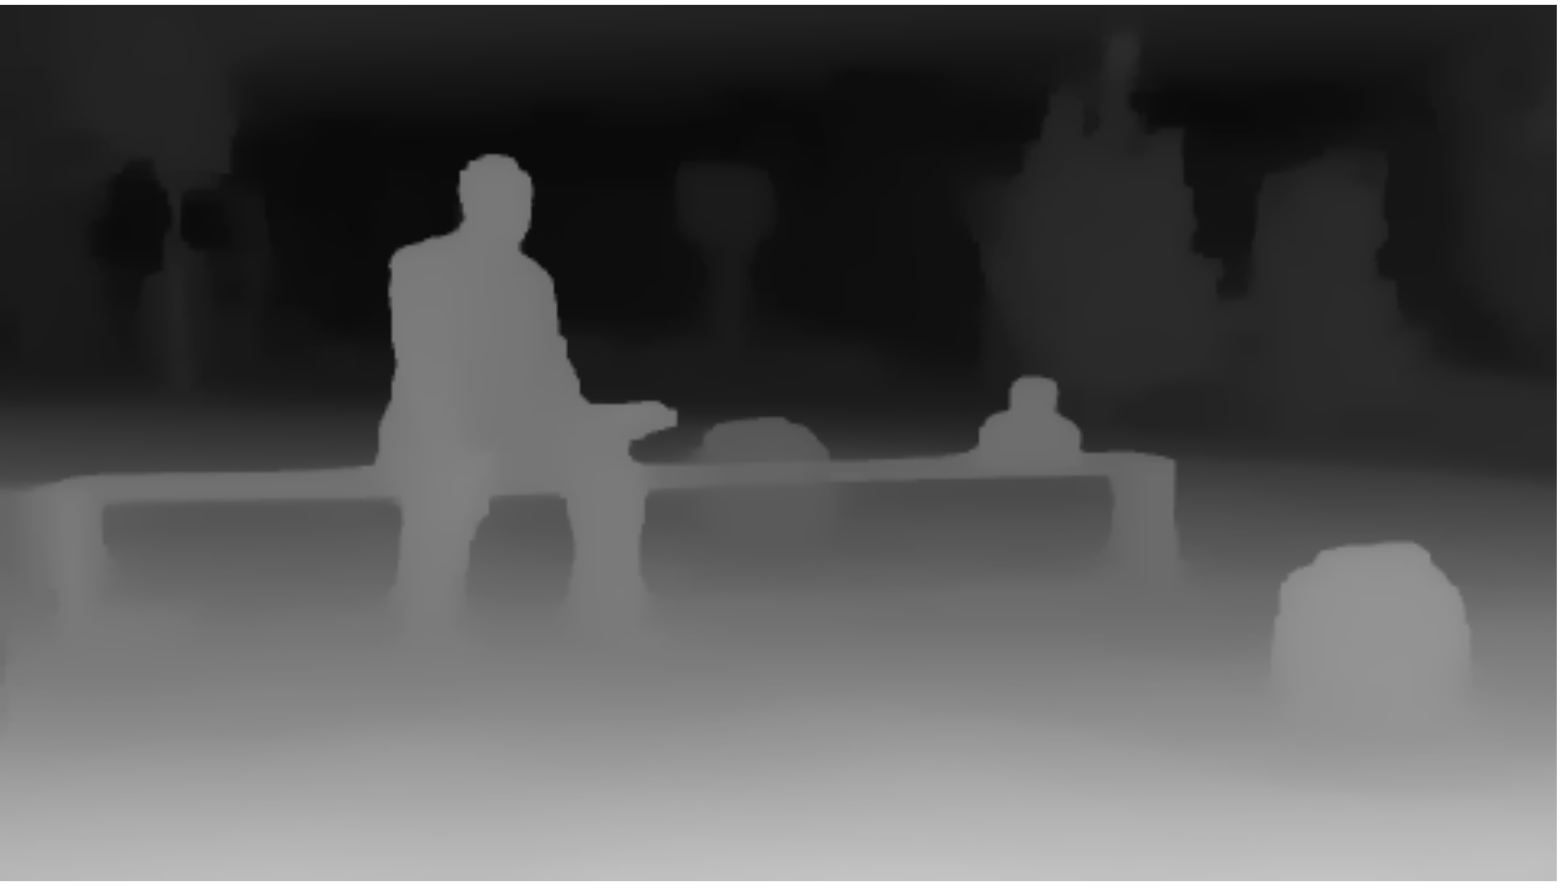
\includegraphics[width=\textwidth]{summary/depthmap_zhang.png}
		%\caption{Caption for image}
	\end{minipage}
	\begin{minipage}[c]{.45\textwidth}
		\centering
		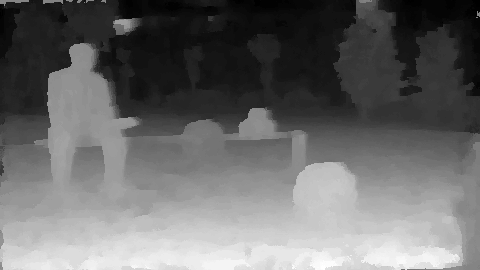
\includegraphics[width=\textwidth]{summary/depthmap_giorgio.png}
		%\caption{Caption for image}
	\end{minipage}
\caption{Comparison between depth-maps estimated using the complete original implementation (left) and depth-maps estimated using the partial implementation provided.}\label{fig:disp_comparison}
\end{figure}

\subsection{Future Work}
A simple improvement over the project could be the implementation of the remaining components. A further expansion to the project could also be the introduction of hardware specific accelerated libraries, such as \Cupy{} or \Pytorch.



\appendix %%%-----------------------------------------------


%%%----------------------------------------------------------
\chapter{Supplementary Algorithms}

\section{Loopy Belief Propagation Algorithm}\label{app:LBP}
\emph{Loopy Belief Propagation} (\LBP) \cite{Felzenszwalb2006} is a dynamic programming algorithm, which can be used to calculate approximate solutions for energy minimization problems defined over labeled graphs. 

\LBP{} is a specialization of the \emph{Belief Propagation} (\Acronym{BP}) algorithm used for {marginal distribution} approximation of \emph{Markov Random Fields}. \LBP{} is able to achieve better performance than regular \Acronym{BP} by making assumptions on the structure of the input graph and energy function.
%Inputs of the \LBP{} algorithm are:
%\begin{itemize}
%	\item A grid graph $\Graph$ with vertices $\Vertices$ and edges $\Edges$. This graph can be used to represent an image; each node is a pixel, and each vertex is connected to the (at  most four) adjacent pixels. 
%	\item An arbitrary finite set of labels $D$. This label set is usually $\{0, ... , n\}$.
%	\item A function $V$ that associates pairs of labels to values in $\R$.
%	\item Two-dimensional table $U$ that associates nodes and labels to values in $\R$. The notation $U_x(d) = \alpha$ with $x\in\Vertices$, $d\in D$, and $\alpha \in \R$ is used to indicate table elements.
%\end{itemize}
%The algorithm can then be used to compute a mapping (denoted as $d_x$) from vertices to labels, such that the following energy function is locally minimized:
%\begin{equation} \label{eq:lbp-example-energy}
%E(\{d_u\}_{u\in\Vertices}) = \sum_{(x,y)\in \Edges} V(d_x,d_y) + \sum_{x\in\Vertices} U_x(d_x) 
%\end{equation}
\subsection{Problem Statement}
Given a graph with vertices (pixels) $P$ and edges $N$, and a set of
labels $L$ (with cardinality $k$), the goal of \LBP{} is to find a 
labeling of the vertices $\{f_{\vec p}\}_{\vec p \in V}$ such that 
the energy function
\begin{equation}\label{eq:lbp:energy}
E\left( \{f_{\vec p}\}_{\vec p \in V}\right) = 
\sum_{(\vec p,\vec q)\in N} V(f_{\vec p},f_{\vec q}) + \sum_{\vec p \in P}  D(\vec p, f_{\vec p})
\end{equation}
is minimized. The terms $V(\cdot,\cdot)$ and $D(\cdot,\cdot)$
are respectively named \emph{discontinuity cost} and \emph{data cost}.
The {data cost} can be any arbitrary mapping between pixel-label pairs
over real values.
On the other hand, the discontinuity cost between two pixels $\vec p$
and $\vec q$ is defined as
\begin{equation}\label{eq:lbp:discontinuity}
V(\vec p, \vec q) = \cdot\min(s \cdot \lVert f_{\vec p} - f_{\vec q}\rVert, \eta),
\end{equation}
with $\eta$ and $s$ positive constants. This restriction allows the discontinuity cost to be computed in a more efficient way.

\subsection{Implementation}
\LBP{} works by iteratively computing a table of messages exchanged between nodes, until convergence is reached or an iteration threshold is exceeded. Each message is a vector of length equal to the number of labels.
Let $m^t_{(\vec p,\vec q)}$ be the message sent by the node $\vec p$ to the adjacent node $\vec q$ at iteration $t$, the content of this message can be recursively described using the messages received by $\vec p$ at time $t-1$, \ie
\begin{equation}\label{eq:lbp:update}
m^t_{(\vec p,\vec q)}(f) = \min_{f'}\left( V(f, f') + D(\vec p, f') + \sum_{s\in N(\vec p) - \vec q} m^t_{(\vec q, \vec s)}(f')\right),
\end{equation}
for each possible label $f\in L$. The set $N(\vec p)-\vec q$ is the set of neighbors of $\vec p$ excluding $\vec q$. The base cases $m^0_{(\vec p,\vec q)}$ are initialized with zero values.
After the desired amount of iterations $T$, it is possible to compute the \emph{belief vector} for ech node $\vec p$ as
$$
b_{\vec p}(f) = D_{\vec p}(f) + \sum_{\vec q\in N(\vec p)} m^T_{(\vec q, \vec p)}(f).
$$
For each node, the final label is the one that minimize the respective belief vector, \ie
$$
f_{\vec p} = \argmin_{f\in L}\left(b_{\vec p}(f)\right).
$$

It is trivial that by alternating two tables of size $|N|\times k$ it is possible to compute the belief vector for each node in the graph, obtaining thus an approximation of the desired graph labeling.

\subsection{Optimizations}
In \cite{Felzenszwalb2006} are described a number of possible optimization that allow the algorithms to execute less computations and reach convergence in less iterations.
Particularly, it is shown an algorithm which allows to compute \cref{eq:lbp:update} linearly to the number of labels by exploiting \cref{eq:lbp:discontinuity}, resulting in the formula
\begin{equation}\label{eq:lbp:update2}
	m^t_{(\vec p,\vec q)}(f) = \min\left(m(f), \min_{f'}\left(h(f'\in L)+\eta\right)\right),
\end{equation}
with the function $h(f')$ defined for every $f'\in L$ as 
\begin{equation}
h(f') =D_{\vec p}(f') + \sum_{\vec s\in N(\vec p) - \vec q} m^{t-1}_{(\vec s, \vec p)}(f')
\end{equation}
and $m(f)$ initialized to $h(f)$ and obtained as result from the procedure
\begin{algorithmic}[0]
	\For{$f=1,\dots,k-1$}
	\State $m(f)\leftarrow \min \left( m(f), m(f-1) + s\right)$
	\EndFor
	\For{$f=k-2,\dots,0$}
	\State $m(f) \leftarrow \min \left( m(f), m(f+1) + s\right)$ 
	\EndFor
\end{algorithmic}
executed "in-place", so that changes are propagated.

%Another possible optimization used to convergence faster, is the Multiscale \LBP{} variant, which create different coarser data costs

\newpage
\section{Conjugate Pixel Computation}\label{app:conjugate_pixel}
\emph{Epipolar geometry} is a branch of mathematics that focuses on stereo vision; it can be used to compute the position of a pixel $\vec x$ with respect to different frames. This new pixel is called "the \emph{conjugate} of $\vec x$", and it is noted as $\vec{x'}$.
Computation of $\vec{x'}$ requires knowledge about the disparity of $\vec x$, noted with $d_{\vec x}$ and use of the camera parameters associated to the respective frames.
%

More precisely, given two frames $t$ and $t'$, the corresponding camera parameters, noted as\footnote{The camera parameters are noted as $\mat K$ for the intrinsic matrix, $\mat T$ for the translation vector, and $\mat R$ for the rotation matrix.} \{$\vec K$, $\vec R$, $\vec T$\},  and \{$\vec{K'}$, $\vec{R'}$, $\vec{T'}$\} respectively, are used to compute $\vec{x'}$, using the formula
$$
\vec{x'}^h = \mat{K'}\Transpose{\mat{R'}}\cdot\left(
\mat R\Inverse{\mat K}\vec x^h + 
d_{\vec x}\cdot\left( \vec T - \vec{T'} \right) \right).$$
Note that $\vec x^h$ denotes the homogeneous coordinates of $\vec x$.
%\begin{figure}[!h]
%	\centering
%	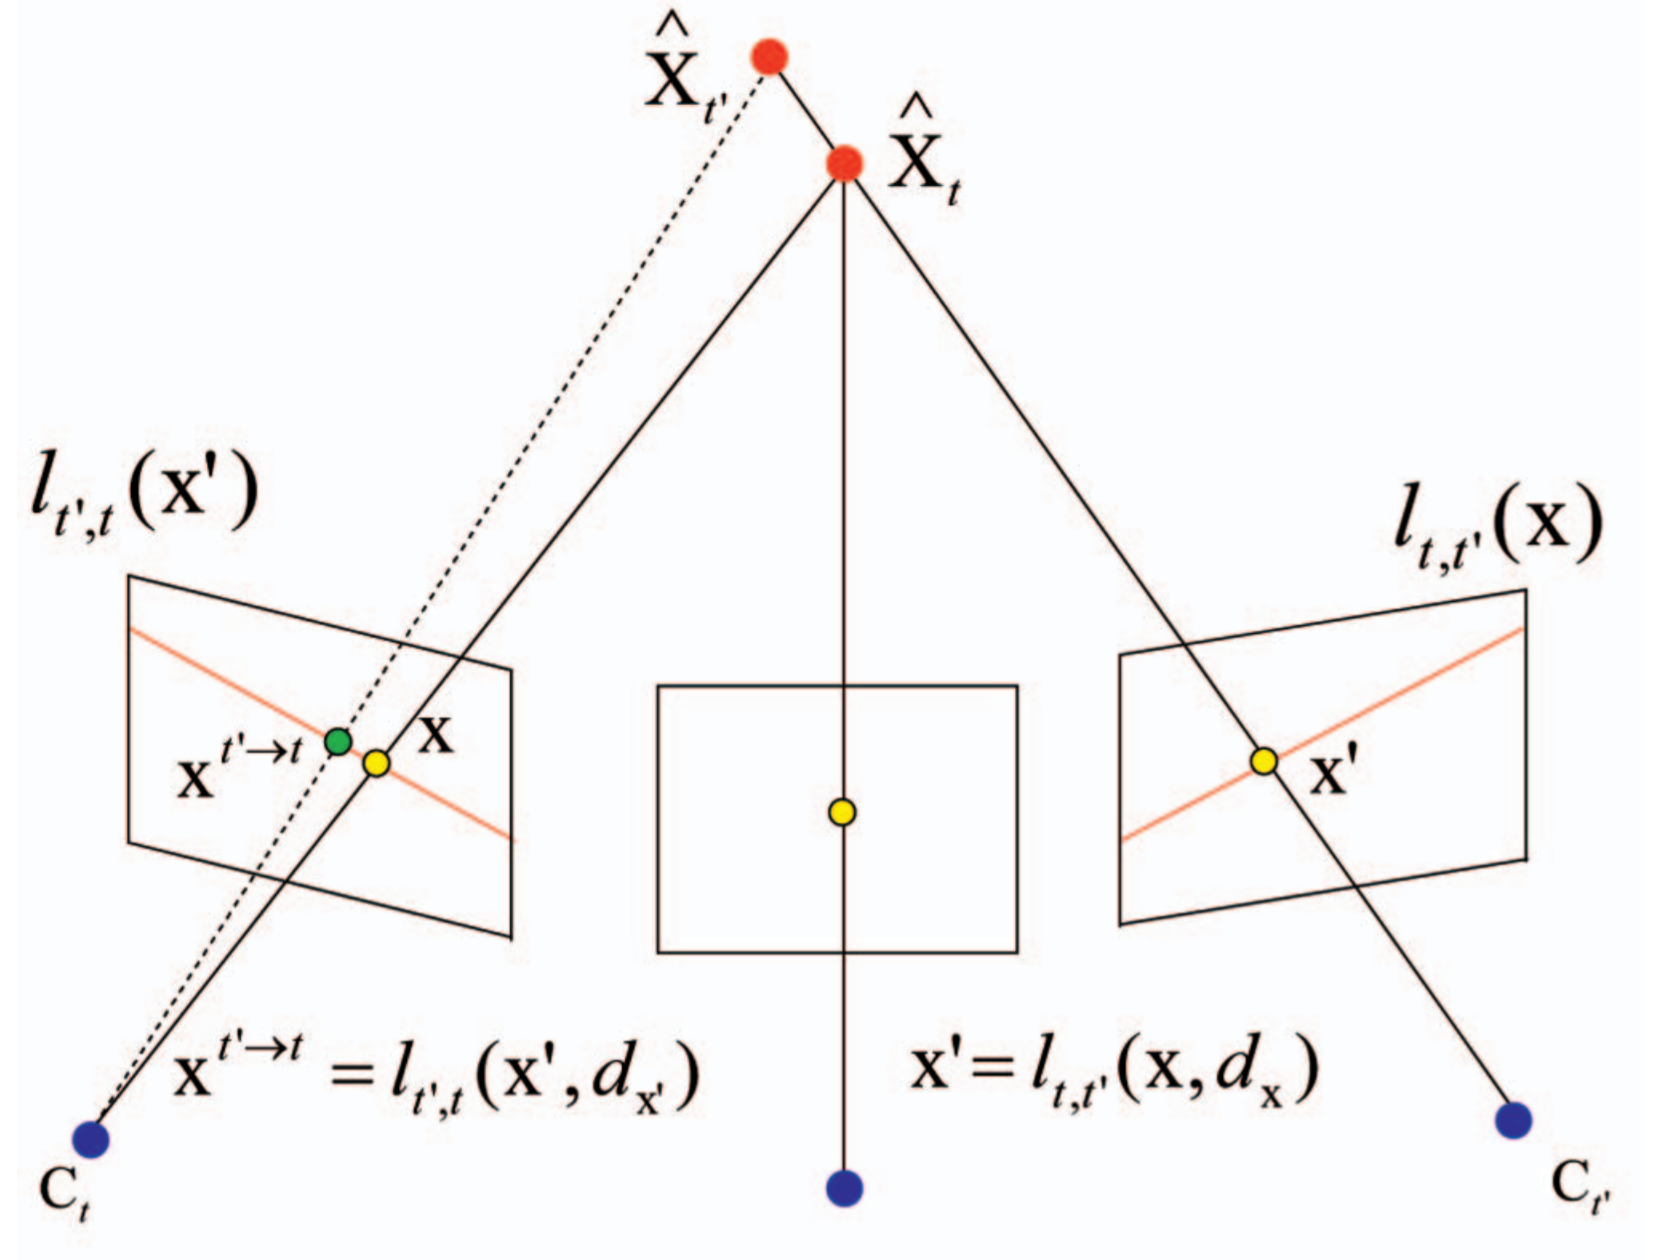
\includegraphics[width=.75\textwidth]{conjugate_pixel.png} %{CS0031}
%	\caption{}
%\end{figure}


%%%----------------------------------------------------------
\MakeBibliography[nosplit]
%%%----------------------------------------------------------


\end{document}
